\chapter{Relativistic Particles in Matter}
\label{ch:cherenkov}
\begin{flushright}
\textit{\\Hofstadter's Law: It always takes longer than you expect, even when you take into account Hofstadter's Law\\}
\end{flushright}

\noindent Charged particles that travel faster than the speed of light in that material produce light in a process that is called the \textit{Cherenkov effect}. The production of photons makes it possible to detect particles with a non-zero charge (electrons, muons, SMPs, etc.) in a neutrino detector such as the IceCube experiment. This cubic-sized detector is able to register the light that is produced from charged particles in air showers and charged particles that are created when neutrinos interact with the ice around or inside the detector. In this chapter, an overview is given of the Cherenkov effect and the different other physical processes that are visible in the IceCube detector. These signatures have to be accounted for in the background prediction when looking for particles with an anomalous charge. Finally, the energy loss formulae of charged particles in matter are given.


\section{Cherenkov effect}
\label{sec:cherenkoveffect}
From Einstein's works on special and general relativity, it follows that the speed of light in vacuum, $c$, is a universal constant. The speed of light in matter can be significantly lower than that. If a particle travels through a dielectric medium at a speed that is greater than the phase velocity of light in that medium, electromagnetic radiation is emitted. This radiation is called \textit{Cherenkov radiation} and is named after the first person who was able to detect it experimentally, Pavel Cherenkov. He was awarded the Nobel Prize in 1958 for his findings together with Frank and Tamm for their theoretical work on the subject \cite{nobel1958url}.

The velocity of a propagating wave is given by the three-dimensional wave equation

\begin{equation}
\nabla^2\psi = \frac{1}{v^2} \frac{\partial^2 \psi}{\partial^2 t},
\end{equation}
where $\psi$ is the wave function and $v$ its group velocity. From Maxwell's equations and some vector calculus, it is straightforward to find that the wave equation for electromagnetic radiation becomes

\begin{equation}
\nabla^2E = \mu \epsilon \frac{\partial^2 E}{\partial^2 t},
\end{equation}
where $E$ is the electric field and $\mu$ and $\epsilon$ the permeability and permittivity of the medium, respectively. From these equations it is clear that for light in a dielectric medium

\begin{equation}
v = \frac{1}{\sqrt{\mu \epsilon}} = \frac{1}{\sqrt{\mu_r \epsilon_r}}\frac{1}{\sqrt{\mu_0 \epsilon_0}} = \frac{1}{\sqrt{\mu_r \epsilon_r}} \times c \leq c,
\end{equation}
where $1/\sqrt{\mu_0 \epsilon_0} = c$ and $\mu_r$ and $\epsilon_r$ are the relative (to vacuum) permeability and permittivity, respectively and are $\geq 1$. These terms are also written as the refractive index of the medium, $n = \sqrt{\mu_r \epsilon_r}$ and result in

\begin{equation}
v = c/n.
\end{equation}

\noindent When a charged particle moves inside a dielectric medium, it excites the molecules of the medium to the higher levels and excited states. The molecules emit photons in the form of electromagnetic radiation upon returning back to their ground state. According to the \textit{Huygens principle}, the emitted waves move out spherically at the phase velocity of the medium (which can be less than the speed of light in vacuum). If the motion of the particle is slow, the radiated waves bunch up slightly in the direction of motion, but they do not cross. However, if the particle moves faster than the light speed, the emitted waves add up constructively, leading to a coherent radiation at angle $\theta_c$ with respect to the particle direction; Cherenkov radiation. The coherent interference is enough to be visible to the naked eye\footnote{The typical blue light in the cooling water at nuclear reactors is also due to this Cherenkov radiation.}. The signature of the effect is a cone of emission in the direction of particle motion. Figure \ref{fig:cherenkov} shows a schematic view of the Cherenkov radiation, illustrating the typical spherical wavefront and the resulting radiation\footnote{The typical cone shape of this effect can be easily seen when observing ducks. If a duck is traveling in a straight line in the water, individual concentric waves can be distinguished and a cone shaped wave is produced behind them.}.

\begin{figure}[ht]
\centering
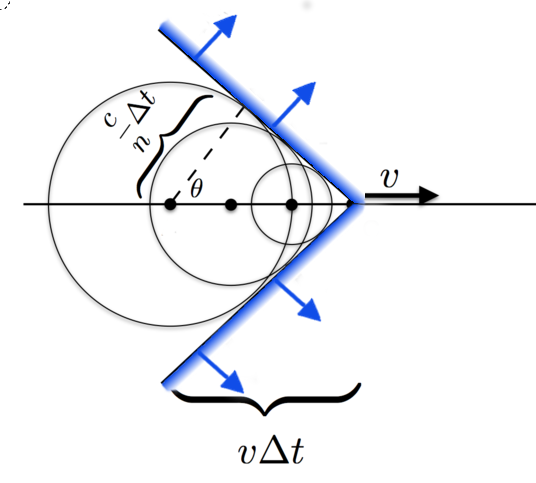
\includegraphics[width=0.6\textwidth]{chapter4/img/cherenkov2.png}
\caption{Schematic view of Cherenkov radiation from a particle traveling at a velocity $v$.}
\label{fig:cherenkov}
\end{figure}

\noindent From the figure we can derive that

\begin{equation}
\cos\theta_c = \frac{\frac{c}{n} \Delta t}{v \Delta t} = \frac{c}{vn} = \frac{1}{\beta n}.
\end{equation} 
Because $-1 \leq \cos\theta_c \leq 1$, the velocity of the charged particle must be $v \geq c/n$. Typical values of $n$ are on the order of 1-2, requiring the particles to be relativistic in order to emit Cherenkov radiation. The number of photons produced per unit path length of a particle with charge $ze$ and per unit energy interval of the photon was calculated by Frank and Tamm, and is often referred to as the Frank-Tamm equation \cite{PDG2018url}

\begin{equation}
\begin{split}
\frac{d^2N}{dE dx} &= \frac{\alpha z^2}{\hbar c} \sin^2 \theta_c = \frac{\alpha^2 z^2}{r_e m_e c^2} \left( 1 - \frac{1}{\beta^2 n^2\left(E\right)} \right)\\
&\approx 370 \sin^2 \theta_c \left(E\right) \textrm{eV}^{-1} \textrm{cm}^{-1} \ \ \ \left( z =1\right),
\end{split}
\end{equation}
where $r_e$ is the classical electron radius, $m_e$ the electron mass and $\alpha$ the fine-structure constant. Equivalently, this equation can be written in function of the wavelength of the photon

\begin{equation}
\label{eq:franktamm}
\frac{d^2N}{dx d\lambda}  = \frac{2\pi \alpha z^2}{\lambda^2} \left(1- \frac{1}{\beta^2 n^2 \left(\lambda \right)} \right),
\end{equation}
where it is clear that the charge of the particle will influence the total Cherenkov light yield. A charge of 1/3$e$ will reduce the light output with a factor of 9 compared to a particle with a charge equal to the electron charge, $e$.\\

\noindent Examples of experiments that make use of this Cherenkov effect are air Cherenkov telescopes such as MAGIC, H.E.S.S and VERITAS that look for the direct and indirect Cherenkov light from gamma rays and cosmic rays. Because the refractive index of air is close to 1 (1.000293 at sea level and smaller with increasing height) the opening angle of the Cherenkov cone is small ($\approx 1^{\circ}$). The particles need to be very relativistic in order for Cherenkov radiation to occur\footnote{Let us assume the refractive index of air at sea level, then, from $E^2/m^2 = \gamma^2 = 1/(1-\beta^2)$, it follows that the minimal energy is $\approx 41$ times its rest mass. Since the refractive index decreases in function of height, the energies of particles interacting with the atmosphere must be even higher.}.

In water and ice, the refractive index is $\approx 1.33$, making $\beta_{min} = 0.75$ and $E_{min} = 1.51 \cdot m_0$. Experiments using water or ice as the interaction medium are Super-Kamiokande, ANTARES and the IceCube experiment.\\

\noindent Most of the light that is emitted from charged particles traveling through matter originates from this Cherenkov effect, provided that their energy is not too high. At higher energies, the amount of secondary particles with an energy high enough to produce Cherenkov effects themselves, becomes so large that this becomes the primary source of light (see Section \ref{sec:energyloss}). This analysis focusses on SMPs that lie below this threshold and we see from Eq. \ref{eq:franktamm} that the charge of the SMP enters in the photon production quadratically. SMPs with a lower charge are therefore expected to produce less photons than minimum ionizing muons.

\section{Neutrino interactions}
\label{sec:neutrinointeractions}
The IceCube experiment is a neutrino detector, but neutrinos have no electromagnetic charge. Neutrinos are only visible through their production of secondary particles with an electromagnetic charge and emit Cherenkov radiation in the ice. Here, we briefly describe how these interactions take place.\\

\noindent Neutrinos interact with matter through both charged current (CC) and neutral current (NC) processes. In the former, the mediator particle is a charged $W$ boson resulting in a charged lepton in the final state. In the latter, the mediator particle is the neutral $Z$ boson. Both interaction types have a resulting hadronic component as daughter particles. The interactions can be written as

\begin{alignat}{2}
\nu_l \left(\bar{\nu}_l\right) + N &\xrightarrow{W} l^- \left(l^+\right) + X^{+\left(-\right)} \ \ && \left(CC\right)\\
\nu_l \left(\bar{\nu}_l\right) + N &\xrightarrow{Z} \nu'_l \left(\bar{\nu}'_l\right) + X && \left(NC\right),
\end{alignat}
where $l$ is the lepton flavor ($e,\mu,\tau$), $N$ denotes the inital hadronic state of the nucleus and $X$ the final hadronic state. These interactions are illustrated in Figure \ref{fig:feynmanneutrino}.\\
\newline
The charged leptons and hadrons lead to light production via gamma ray production and Cherenkov radiation. With the right material, it is possible to detect this light production and reconstruct some of the neutrino's characteristics. \textcolor{red}{Because the light production depends on the square of the charge of a particle, the IceCube detector is not powerful in detecting if the primary particle was a neutrino or antineutrino\footnote{Although it is not possible to distinguish neutrino from antineutrino events on an event-by-event basis, there are ways to look at differences. One example is to look at inelasticity effects as done in Ref. \cite{Aartsen:2018vez}.}.}

\begin{figure}[t]
\centering
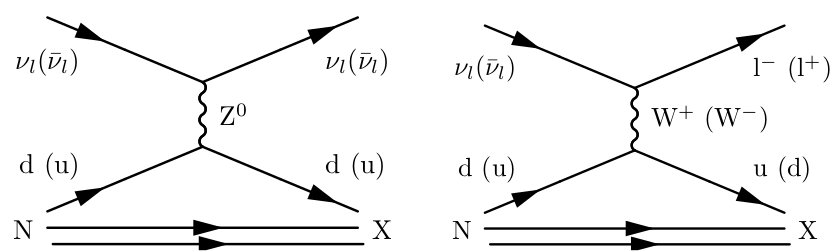
\includegraphics[width = 0.9\textwidth]{chapter4/img/feynmanneutrino.png}
\caption{Feynman diagrams of NC (\textit{left}) and CC (\textit{right}) neutrino interactions. $l$ is the lepton flavor ($e,\mu,\tau$), $N$ denotes the intial hadronic state of the nucleus and $X$ the final hadronic state. The antineutrino interactions are given in brackets.}
\label{fig:feynmanneutrino}
\end{figure}


\section{Propagation}
\label{sec:propagation}
As described in Section \ref{sec:neutrinointeractions}, neutrinos give rise to several types of interactions in the surrounding medium. There are three characteristic signatures, which are the main interest in the IceCube detector (illustrated in Figure \ref{fig:ICinteractions}).

\begin{figure}[t]
\centering
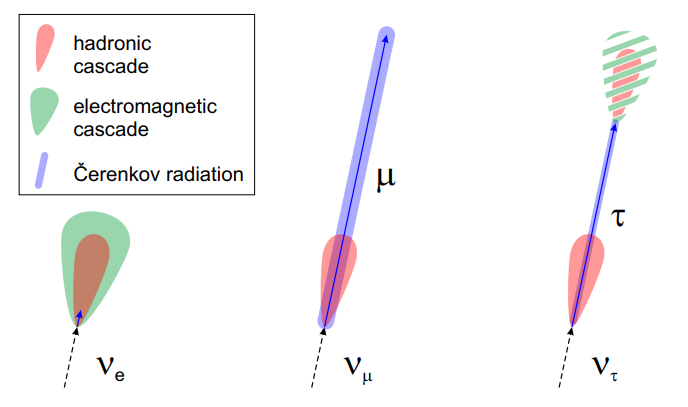
\includegraphics[width=0.7\textwidth]{chapter4/img/ICinteractions.png}
\caption{Schematic view of the neutrino signatures in matter. At each interaction point there is a hadronic cascade (red). Every hadronic cascade has electromagnetic sub-showers which are not illustrated here. Muons and energetic taus can give rise to tracks. The electromagnetic and hadronic cascades have a more spherical shape but are exaggerated for illustrative purposes in the figure. Illustrations from Ref. \cite{Wallraff}.}
\label{fig:ICinteractions}
\end{figure}

\subsection{Cascades}
\subsubsection{Electrons and photons}

In a charged current neutrino interaction, the energetic electron gives rise to a shower of gamma rays (bremsstrahlung) and positrons and electrons (pair production). Positrons and electrons in their turn emit new gamma rays and this process continues until the photon energies fall below the pair production threshold. Because electrons/positrons lose their energy fast, they are almost immediately stopped, giving an \textit{electromagnetic cascade} an almost spherical shape.

Let us assume $E_0$ is the energy of the incoming electron. In a very simplistic toy model one can say that an electron emits one photon after one radiation length, $X_0$. A photon will decay into an electron-positron pair after approximately one radiation length too\footnote{In fact one radiation length implies $1/e$ times the initial energy. Assuming the electron loses half its energy to the photon, then 0.63/0.5 $\approx 1$. After one radiation length, a high energy photon loses $\approx 7/9$ times its energy via bremsstrahlung, again we assume $\approx 1$.}. At every decay or radiation process, it is assumed that the daugher particles carry 1/2 of the energy. After $t$ steps, the energy is equal to

\begin{equation}
E(t) = \frac{E_0}{2^t}.
\end{equation}
The number of particles will be equal to

\begin{equation}
N(t) = 2^t.
\end{equation}
At a critical energy $E_c$, the multiplication process stops (as pair production dominates over bremsstrahlung) and we find

\begin{equation}
t_{max} = \frac{\ln\left(\frac{E_0}{E_c}\right)}{\ln 2},
\end{equation}
the total longitudinal length of an electromagnetic shower is thus approximately equal to

\begin{equation}
X = X_0 \frac{\ln\left(\frac{E_0}{E_c}\right)}{\ln 2}.
\end{equation}
This logarithmic dependence on the energy of the initial particle will therefore result into elongations of a couple of meters at most. Typical values in ice are $X_0 \approx 40$ cm and $E_c \approx 80$ MeV.

\subsubsection{Hadrons}
In the case of neutral current events, the breakup of the struck nucleus leads to charged byproducts. These byproducts can reinteract in the medium and produce neutral pions that decay into gamma rays. These particles again die out quickly, resulting in a spherical emission of light for \textit{hadronic cascades}. The basic development of hadronic cascades in space is very similar to that of electromagnetic ones, but with important differences in energy loss, particle content, lateral spread and fluctuations. Hadronic cascades contain particles heavier than electrons, that have a higher Cherenkov threshold. A fraction of them are slow neutrons, which do not produce any light. Neutral pions produce gamma rays. Charged pions, on the other hand, can decay into muons and muon neutrinos; long-ranged particles that do not contribute to the cascading process. Finally, a non-neglibible fraction of the energy is lost in the hadronic binding processes.

The light yield will be smaller than the one obtained from an electromagnetic cascade of equal initial energy and with much larger event-by-event variations. 


\subsection{Muon tracks}
Muons are produced in charged current muon-neutrino interactions and travel much further than electrons and positrons. The relativistic muon will produce light according to the Frank-Tamm equation, Eq. \ref{eq:franktamm}, resulting in \textit{direct Cherenkov radiation}. Ionization, bremsstrahlung, pair production, and photonuclear interactions (see Section \ref{sec:energyloss}) are also capable of producing relativistic secondary particles that produce \textit{indirect Cherenkov radiation}. Both effects result in a Cherenkov cone with a diffuse light emission from the track in all directions behind it. 

\subsubsection{Energy loss}
\label{subsub:energyloss}
Below 1 TeV, muons will lose most of their energy to ionization losses. A charged particle traversing matter ionizes the material around it. When the energy transfer is high enough, electrons can be stripped away from their atoms, resulting in \textit{delta electrons}. As can be seen in Figure \ref{fig:energyloss}, ionization losses have only a very weak energy dependence. It is therefore very difficult to distinguish for example a 50 GeV from a 500 GeV muon as the direct Cherenkov light production will be similar (Eq. \ref{eq:franktamm}) and the energy loss is from the almost-energy-independent ionization.

Above 1 TeV, however, the muon, on average, loses more energy to stochastic\footnote{In this context we mean that the energy losses are not deterministic: it is impossible to know when an interaction of this kind will occur. One can only make estimations of their \textit{expected} effects.} effects. Here, effects such as bremsstrahlung, pair production and the photonuclear effect dominate over ionization (see Section \ref{sec:energyloss}). Therefore, indirect Cherenkov production starts to dominate and makes the energy estimation much easier.\\

\begin{figure}[t]
\centering
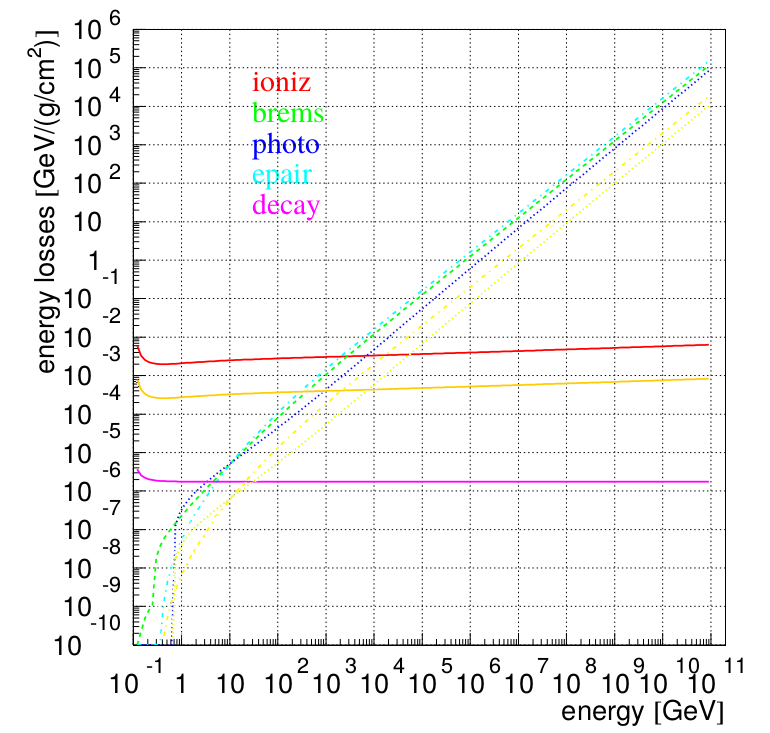
\includegraphics[width = 0.7\textwidth]{chapter4/img/muonenergyloss_extra.png}
\caption{Muon energy loss from ionization (upper solid curve, red), bremsstrahlung (dashed, green), photonuclear (dotted, blue), pair production (dashed-dotted, cyan) and decay (lower solid curve, purple). Additionally, the expected energy losses of a muon with charge 1/3 are shown in orange/yellow. Ionization, photonuclear and pair production scale with $z^2$, giving a factor 9 difference. Bremsstrahlung, which has a $z^4$ dependence is left out.}
\label{fig:energyloss}
\end{figure}

\noindent The average energy loss from ionization and stochastic effects along the muon trajectory can be parametrized by \cite{Barrett:1952woo} 

\begin{equation}
\label{eq:energyloss}
- \frac{dE}{dx} = a + b \cdot E_\mu,
\end{equation}
where $a$ and $b$ are obtained by fitting and can be found in Table \ref{tab:energylossconstants}. Here $a$ corresponds to the ionization energy loss (given by Eq. \ref{eq:ioniz}), and $b$ corresponds to the sum of $e^+e^-$ pair production, bremsstrahlung, and photonuclear contributions. The muon range can be found by integrating Eq. \ref{eq:energyloss}

\begin{equation}
\begin{split}
R_\mu \approx \frac{1}{b} \ln \left( \frac{E_\mu}{E_{th}} +1 \right),
\end{split}
\end{equation}
with $E_{th} = a/b = 720$ GeV, the energy theshold above which stochastic effects are dominant.\\


% Please add the following required packages to your document preamble:
% \usepackage[table,xcdraw]{xcolor}
% If you use beamer only pass "xcolor=table" option, i.e. \documentclass[xcolor=table]{beamer}
\begin{table}[]
\caption{Best fits for muon energy loss parameters $a$ and $b$ from Eq. \ref{eq:energyloss}. Fits from Ref. \cite{Chirkin:2004hz}.}
\label{tab:energylossconstants}
\begin{center}
\begin{tabular}{|l |c|c|}
\hline
{\cellcolor[HTML]{F1A91E} \textbf{Medium}}   & \cellcolor[HTML]{F1A91E}{$a \left(\frac{\textrm{GeV}}{\textrm{mwe}}\right)$} & \cellcolor[HTML]{F1A91E}{$b \left(\frac{10^{-3}}{\textrm{mwe}}\right)$} \\ \hline 
\textbf{Air}    & 0.281                                                                                             & 0.347                                                                                        \\ \hline
\textbf{Ice}      & 0.259                                                                                             & 0.363                                                                                        \\ \hline
\textbf{Fr. Rock} & 0.231                                                                                             & 0.436                                                                                        \\ \hline
\textbf{St. Rock} & 0.223                                                                                             & 0.463                                                                                        \\ \hline
\end{tabular}
\end{center}
\centering ${}^\dagger$ Mwe stands for ``meter water equivalent'', a unit often used in cosmic ray physics. A detector shielded by matter equal to 100 mwe would be equally shielded from cosmic rays if it were 100 meters below water.
\end{table}

\noindent SMPs will have very similar signatures in the IceCube detector as we have assumed that they behave leptonically (Section \ref{sec:properties}). The tracks will be dim compared to muon tracks due to the charge dependence in the Cherenkov effect (Section \ref{sec:cherenkoveffect}).

\section{Energy loss formulae}
\label{sec:energyloss}
As mentioned in Section \ref{subsub:energyloss}, secondary interactions such as bremsstrahlung, pair production and photonuclear effect, become non-negligible at certain energies. At high energies (> 1 TeV for muons) the Cherenkov light of the secondary particles will have a significant contribution additional to the Cherenkov light coming from the primary particle. These effects are taken into account in IceCube simulations and are of great importance for high-energy muons. Since these interactions are electromagnetic in nature, they will also play a role for SMP particles, yet these effects are small for the SMPs with a primary focus on lower energies.

In this section we go over the four main components of secondary interactions. This section is largely based on the findings in Ref. \cite{Chirkin:2004hz}. The energy of the secondary particles will be expressed by $\nu = v E$, with $E$ the energy of the incident particle and $v$ the fraction of the energy transfer. Secondary interactions occur at all energy levels and become continuous in nature below a certain energy threshold. Therefore, in many codes $v_{cut}$ is implemented as a lower bound equal to 0.05 and a $\nu_{cut}$ equal to 500 MeV \cite{dimaspice}. 

\subsection{Ionization}
Fast charged particles that move through matter interact with the electrons of atoms in the material. The interaction excites or ionizes the atoms. The Feynman diagram of this interaction is given in Figure \ref{fig:feynmanionizbrems} (left). 

The cross section is expressed as 

\begin{equation}
\begin{split}
\frac{d^2N}{d\nu dx} = &\frac{1}{2} K z^2 \frac{Z}{A} \frac{1}{\beta^2} \frac{1}{
\nu^2} \left[1-\beta^2 \frac{\nu}{\nu_{max}} + \frac{1}{2} \left(\frac{\nu}{E(1+1/\gamma)} \right)^2 \right],\\
&\textrm{with   } \nu_{max} = \frac{2 m_e (\gamma^2 -1)}{1+2\gamma \frac{m_e}{m_t} +\left(\frac{m_e}{m_t}\right)^2}
\end{split}
\end{equation}
where negligible terms are left out and $K$ is equal to $4\pi N_A r_e^2 m_e c^2$, $N_A$ is Avogadro's number, $r_e$ the classical electron radius, $m_e$ the electron mass, $z$ the charge of the particle (in units of the electron charge), $Z$ the atomic number of the absorber, $A$ the atomic mass of the absorber and $m_t$ the mass of the throughgoing particle.

This interaction leads to an energy loss of the traveling particle and is expressed by the Bethe-Bloch formula \cite{PDG2018url}

\begin{equation}
\label{eq:ioniz}
\begin{split}
-\left\langle\frac{dE}{dx}\right\rangle = K z^2 \frac{Z}{A \beta^2} &\left[\frac{1}{2} \ln \left(\frac{2 m_e \beta^2 \gamma^2 \nu_{upper}}{I\left(Z\right)^2} \right) -\frac{\beta^2}{2}  \left(1+\frac{\nu_{upper}}{\nu_{max}} \right) + \frac{1}{2} \left( \frac{\nu_{upper}}{2E(1+1/\gamma)}\right)^2 - \frac{\delta}{2}\right], \\ 
&\textrm{where } \nu_{upper} = \min(\nu_{cut},\nu_{max}) 
\end{split}
\end{equation} 
where $I$ is the mean excitation energy of the absorber. The density correction $\delta$ can be found in the corresponding literature \cite{Chirkin:2004hz}.

For particles in the region of $0.1 \leq \beta \gamma \leq 1000$ this is the dominant factor in the mean energy loss. 

\begin{figure}
\centering
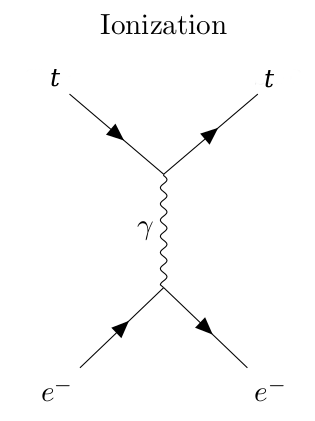
\includegraphics[width = 0.35\textwidth]{chapter4/img/Feynman_Ionization_2.png}
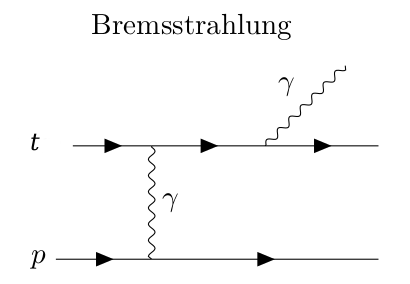
\includegraphics[width = 0.48\textwidth]{chapter4/img/Feynman_Bremsstrahlung_2.png}
\caption{Feynman diagrams of an ionization interaction (\textit{left}) and bremsstrahlung (\textit{right}). \textit{t} denotes the primary particle.}
\label{fig:feynmanionizbrems}
\end{figure}


\subsection{Bremsstrahlung}
Charged particles that decelerate by another charged particle lose kinetic energy that is converted into radiation. This phenomena is known as \textit{bremsstrahlung} and is illustrated in Figure \ref{fig:feynmanionizbrems} (right). The cross section may be represented by the sum of an elastic component and two inelastic components,

\begin{equation}
\sigma = \sigma_{el} + \Delta \sigma^{in}_a + \Delta \sigma^{in}_n,
\end{equation}
where $\sigma_{el}$ denotes the cross section for the Coulomb scattering of the particle off the atomic nucleus and the two other terms are corrections that account for additional processes, in which the bremsstrahlung is accompanied by a change of electron or nuclear structure of the atom in the final state.

\subsubsection{Elastic component}
\begin{equation}
\begin{split}
\sigma_{el} (E,v) = \frac{ \alpha}{v} \left(2 z^2 Z \frac{m_e}{m_t} r_e\right)^2
 &\left(\frac{4}{3} - \frac{4}{3}v +v^2 \right) \left[\ln \left[\frac{m_t}{\delta}\right] - \frac{1}{2} - \Delta \sigma^{el}_a -\Delta \sigma^{el}_ n \right],\\
& \textrm{ \ \ where \ \ } \delta \approx \frac{\mu^2 \omega}{2E(E-\omega)},
\end{split}
\end{equation}
where $\alpha$ is the fine structure constant and $\omega$ the photon's frequency with $\hbar = 1$. The atomic and nuclear formfactors are equal to

\begin{equation}
\label{eq:formfactors}
\begin{split}
&\Delta \sigma^{el}_a(\delta) = \left[ 1+ \frac{1}{\delta \sqrt{e} BZ^{-1/3}/m_e}\right] \\
&\Delta \sigma^{el}_n(\delta) = \left[\frac{D_n}{1+\delta (D_n \sqrt{e} -1)/m_t}\right].
\end{split}
\end{equation}
Values for $B$ and $D_n$ can be found in Ref. \cite{Kelner:1995hu}, here, $e$ is the base of the natural logarithm ($\approx 2.718$) and other constants are as defined in Eq. \ref{eq:ioniz}. Other parametrizations can be found in the corresponding literature \cite{Chirkin:2004hz}. 
%mu hier dimensieloos (zie inleiding)

\subsection{Inelastic component}

The effect of nuclear excitation can be evaluated as

\begin{equation}
\Delta \sigma^{in}_n = \frac{1}{Z} \Delta \sigma^{el}_n; (Z \neq 1),
 \end{equation}
where $\Delta \sigma^{el}_n$ is defined in Eq. \ref{eq:formfactors}.

In the case of atomic excitation, one accounts for bremsstrahlung whereby photons radiate from the primary particle and where photons radiate from the electrons of the atom. This factor is equal to

\begin{equation}
\Delta \sigma^{in}_a \approx \frac{1}{Z} \ln \left[ \frac{m_t/\delta}{\delta m_t/m_e^2 + \sqrt{e}} \right] - \ln\left[1+ \frac{m_e}{\delta \sqrt{e} B' Z^{-2/3}} \right],
\end{equation}
where $B'=1429$ for $Z > 2$, $B' = 446$ for $Z=1$ and $e$ is again the base of the natural logarithm.
\subsection{Photonuclear}
The photonuclear interaction of leptons is the process by which a lepton scatters inelastically with a nucleon or nucleus. Through a virtual photon exchange, hadrons are produced, as is illustrated in Figure \ref{fig:feynmannuclpairprod} (left). The cross section formula is given by

\begin{equation} 
\begin{split} 
\frac{d\sigma}{dv} &= \frac{z^2 \alpha}{2\pi} A \sigma_{\gamma N} v  \Bigg \lbrace  0.75 G(x) \Bigg [\kappa \ln \left(1+\frac{m_1^2}{t}\right) \\
& -\frac{\kappa m_1^2}{m_1^2 + t} - \frac{2 m_t^2}{t} + \frac{4 m_t^2}{m_1^2} \ln \left(1+ \frac{m_1^2}{t} \right)  \Bigg] \\
& + 0.25 \left[ \left(\kappa + \frac{2m_t^2}{m_2^2} \right) \ln \left(1+\frac{m_2^2}{t} \right) - \frac{2m_t^2}{t}\right]\\
& + \frac{m_t^2}{2t} \left[ 0.75 G(x) \frac{m_1^2 -4t}{m_1^2 +t} +0.25 \frac{m_2^2}{t} \ln \left(1+\frac{t}{m_2^2} \right) \right] \Bigg \rbrace,\\
& \textrm{where \ \ } t = Q_{max}^2 = \frac{m_t^2 v^2}{1-v}, \ \ \kappa = 1-\frac{2}{v} + \frac{2}{v^2}, \\
& m_1^2 = 0.54 \textrm{ GeV}^2, \ \ \textrm{and \ \ \ } m_2^2 = 1.8 \textrm{\ GeV}^2.
\end{split} 
\end{equation}
Parameters that aren't defined here can be found in the corresponding literature \cite{Chirkin:2004hz}.

%\begin{equation}
%\sigma_{\gamma N}
%\end{equation}
\subsection{Pair production}
\label{subsec:pairprod}
Pair production occurs when the virtual photon radiated from the primary particle or proton splits into an electron-positron pair or muon-antimuon pair, as is illustrated in Figure \ref{fig:feynmannuclpairprod} (right). The differenctial cross section is equal to
 
\begin{equation}
\begin{split}
&\frac{d\sigma(E,v,\rho)}{dvd\rho} = \frac{2}{3\pi} Z(Z+\zeta)(z \alpha r_e)^2 \frac{1-v}{v} \left(\Phi_e + \frac{m_e^2}{m_\mu^2} \Phi_\mu \right), \\
& \textrm{ where \ \ } v = (\epsilon_+ + \epsilon_-)/E, \ \ \rho = (\epsilon_+ - \epsilon_-)/(\epsilon_+ + \epsilon_-),
\end{split}
\end{equation}
and $\epsilon_+$ and $\epsilon_-$ denote the energies of the positively and negatively charged electrons/muons. The parameters not described in detail can be found in the corresponding literature \cite{Chirkin:2004hz}.

\begin{figure}
\centering
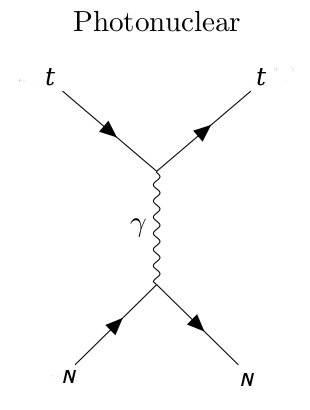
\includegraphics[width = 0.35\textwidth]{chapter4/img/Feynman_PhotoNuclear_2.png}
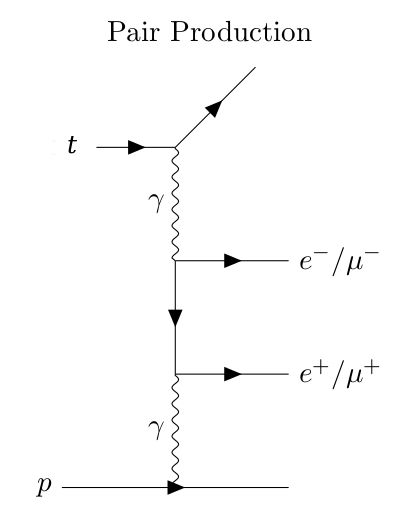
\includegraphics[width = 0.35\textwidth]{chapter4/img/Feynman_PairProduction_2.png}
\caption{Feynman diagrams of a photonuclear interaction (\textit{left}) and pair production (\textit{right}). $t$ denotes the primary particle.}
\label{fig:feynmannuclpairprod}
\end{figure}

\subsection{Conclusion}
\label{sub:energylossconclusion}
From the previous discussion we can conclude that the charge enters in the energy loss formulae quadratically for ionization, pair production and the photonuclear effect. Bremsstrahlung scales with a factor of $z^4$, making it negligible compared to the other energy losses. The influence of the mass of the particle enters these equations in a non-trivial manner but has a minimal effect, again with brensstrahlung as the exception. There, the mass enters with $1/m^2_t$, making it completely negligible for heavy particles. The effects from secondary particle production in the light yield are only substantial at very relativistic SMPs ($\approx 10^4$ times the rest mass). Due to the assumed $E^{-2}$ signal flux (see Chapter \ref{ch:theoreticalmotivation}), their relative contribution to the sample is very small but accounted for.
